\documentclass[conference]{IEEEtran}
\IEEEoverridecommandlockouts

\usepackage{cite}
\usepackage{amsmath,amssymb,amsfonts}
\usepackage{algorithmic}
\usepackage{graphicx}
\usepackage{textcomp}
\usepackage{xcolor}
\usepackage{float}
\usepackage{booktabs}
\usepackage{url} 
\usepackage[utf8]{inputenc}
\usepackage[T1]{fontenc}
\usepackage[brazilian]{babel}
\addto\captionsbrazilian{\renewcommand{\abstractname}{Abstract}}
\usepackage{hyperref}
\usepackage{tikz}
\usetikzlibrary{positioning, arrows.meta}

\begin{document}
\raggedbottom

\title{Manutenção Preditiva no Sistema de Pressão de Ar de Veículos Pesados: Uma Abordagem Sensível ao Custo Baseada em Aprendizado de Máquina}

\author{
    \IEEEauthorblockN{João Vitor Lobato Romualdo}
    \IEEEauthorblockA{
        \textit{Departamento de Computação}\\
        \textit{Centro Federal de Educação Tecnológica de Minas Gerais (CEFET-MG)}\\ 
        Campus V -- Divinópolis, Brasil \\
        joaovitorlobatoromualdo16@gmail.com}
}

\maketitle

\begin{abstract}
A manutenção preditiva em frotas de transporte pesado é determinante para assegurar a confiabilidade operacional e conter custos logísticos decorrentes de paradas não planejadas. Este trabalho propõe e avalia experimentalmente um arcabouço metodológico de aprendizado de máquina sensível ao custo voltado ao diagnóstico de falhas relacionadas ao Sistema de Pressão de Ar (\textit{Air Pressure System} -- APS) de caminhões comerciais, utilizando a base de dados pública \textit{APS Failure at Scania Trucks} (60.000 instâncias de treino e 16.000 de teste, com 170 atributos e cerca de 1,8\% de casos positivos). Contrastam-se a Regressão Logística com ponderação de classes (\textit{baseline} transparente e leve) e comitês de Árvores de Decisão (\textit{Random Forest}) sob validação cruzada estratificada de 5 dobras sem vazamento de dados. Na configuração de referência (custo oficial de \$10 por falso positivo e \$500 por falso negativo), a otimização de limiar \textit{out-of-fold} reduz o custo de teste da \textit{Random Forest} de \$76.660 ($\theta=0{,}50$) para \$10.260 ($\theta_{OOF}=0{,}04$; \textit{Recall} de 97,07\%), superando a Regressão Logística (\$14.450 em $\theta_{OOF}=0{,}39$; \textit{Recall} de 94,67\%). Ampliando a investigação, demonstra-se que: (i) a superioridade da \textit{Random Forest} mantém-se estável em cinco estratégias de tratamento de dados ausentes, e a adição de indicadores binários de ausência (\textit{missingness indicators}) reduz o custo para \$9.450 na \textit{Random Forest} e \$12.910 na Regressão Logística; (ii) a calibração de probabilidades (\textit{Platt Scaling} e Regressão Isotônica) corrige a severa distorção induzida pela ponderação de classes na Regressão Logística (reduzindo o Brier Score de $0{,}0218$ para $0{,}0088$ e o custo sob o limiar teórico de Bayes $\theta^*=0{,}0196$ de \$144.180 para \$14.340) e permite que a \textit{Random Forest} calibrada por Platt atinja \$8.410; e (iii) a análise de sensibilidade à razão de custos ($\rho = c_{FN}/c_{FP} \in [10, 200]$) evidencia que o sobrecusto relativo do modelo linear interpretável cresce de 1,23$\times$ ($\rho=10$) para 2,06$\times$ ($\rho=200$).
\end{abstract}

\begin{IEEEkeywords}
Manutenção Preditiva, Aprendizado de Máquina, Sistema de Pressão de Ar, Aprendizado Sensível ao Custo, Calibração de Probabilidades, Imputação de Dados Ausentes.
\end{IEEEkeywords}

% =========================================================================
% SEÇÃO I: INTRODUÇÃO (REVISADA SEGUNDO FEEDBACK DOCENTE - SEM SUBSEÇÕES)
% =========================================================================
\section{Introdução}

A manutenção automotiva em frotas comerciais de transporte de carga representa um dos pilares mais sensíveis para a sustentabilidade operacional e a segurança viária na indústria logística. Historicamente, a gestão da integridade veicular esteve ancorada em dois paradigmas convencionais: a manutenção corretiva, realizada após a quebra do componente e caracterizada por reboques caros e atrasos na cadeia de suprimentos, e a manutenção preventiva estática, guiada por intervalos fixos de quilometragem que frequentemente substituem peças ainda funcionais ou falham em antecipar quebras prematuras. Com o advento da telemetria embarcada e da conectividade em tempo real, a Manutenção Preditiva (\textit{Predictive Maintenance} -- PdM) emergiu como uma abordagem capaz de monitorar continuamente sinais de sensores veiculares, permitindo estimar a saúde mecânica dos subsistemas e intervir precisamente antes da ocorrência de avarias críticas~\cite{hector2024predictive}.

No estado da arte do monitoramento veicular, técnicas de Aprendizado de Máquina (\textit{Machine Learning} -- ML) têm sido crescentemente empregadas na análise de séries temporais e dados tabulares de sensores. As soluções reportadas na literatura abrangem desde regressores e classificadores supervisionados tradicionais até redes neurais profundas para prognóstico de falhas em sistemas como turbinas aeronáuticas~\cite{rengasamy2020deep}. Modelos baseados em árvores de decisão e comitês de árvores, em particular, alcançaram destaque prático devido à sua habilidade em modelar não-linearidades e processar variáveis heterogêneas sem a exigência de premissas distribucionais rígidas~\cite{gondek2016prediction,cerqueira2016combining}.

Não obstante tais progressos, as soluções de melhor desempenho no \textit{benchmark} de custo da Scania tendem a depender de comitês complexos e de engenharia manual de atributos~\cite{costa2016ida,gondek2016prediction,cerqueira2016combining}, e o custo de abrir mão de modelos mais simples e interpretáveis raramente é quantificado de forma sistemática. Mais ainda, a literatura sobre manutenção preditiva no conjunto da Scania costuma fixar uma única regra de imputação de dados faltantes, operar diretamente sobre escores ou probabilidades não calibradas distorcidas pelo balanceamento de classes e avaliar o desempenho apenas sob a razão de custos estática de $50:1$ (\$500 por falso negativo contra \$10 por falso positivo)~\cite{scania_dataset}. Na operação industrial concreta, entretanto, três questões interligadas desafiam a robustez dessas conclusões: (i) os valores omissos em sensores automotivos frequentemente não ocorrem de forma completamente aleatória, podendo refletir a ausência de determinados sensores em variantes de chassi ou falhas de leitura, de modo que escolhas arbitrárias de descarte e imputação podem alterar a estabilidade comparativa dos modelos~\cite{rafsunjani2019}; (ii) o uso de ponderação de classes (\texttt{class\_weight}) ou de comitês de árvores distorce as estimativas probabilísticas posteriores~\cite{zadrozny2002transforming,niculescu2005predicting,dalpozzolo2015calibrating}, dissociando o limiar ótimo empírico do limiar ótimo teórico de Bayes~\cite{elkan2001foundations}; e (iii) a razão entre o custo de uma avaria em rota e o custo de uma inspeção preventiva varia conforme contratos logísticos, severidade de rota e disponibilidade de oficina~\cite{drummond2006cost,hughes2025xai}.

Para preencher essa lacuna, este trabalho propõe um arcabouço experimental comparativo voltado ao diagnóstico de falhas no Sistema de Pressão de Ar (\textit{Air Pressure System} -- APS) de caminhões pesados, empregando o benchmark público \textit{APS Failure at Scania Trucks Dataset}~\cite{scania_dataset}. Contrastam-se a Regressão Logística com ponderação de classes (como \textit{baseline} linear transparente e adequado a sistemas embarcados) e comitês de Árvores de Decisão (\textit{Random Forest}). Diferentemente de análises restritas ao ponto nominal de operação, a proposta investiga a estabilidade das conclusões sob diferentes estratégias de tratamento de atributos ausentes, incorpora técnicas de calibração de probabilidades (\textit{Platt Scaling} e Regressão Isotônica) aliadas à otimização de limiar \textit{out-of-fold} e realiza uma análise abrangente de sensibilidade aos custos atribuídos aos erros.

O presente documento estrutura-se da seguinte forma: a Seção~\ref{sec:trabalhos_relacionados} delineia a Revisão da Literatura, examinando os estudos correlatos no APS Failure e a fundamentação sobre imputação, calibração probabilística e sensibilidade ao custo; a Seção~\ref{sec:metodologia} detalha os Materiais e Métodos, descrevendo a base de dados, os regimes de tratamento de dados ausentes, os modelos avaliados, os procedimentos de calibração e análise de sensibilidade aos custos e o fluxograma metodológico; a Seção~\ref{sec:resultados} apresenta e discute criticamente os resultados experimentais obtidos; e a Seção~\ref{sec:conclusoes} consolida as conclusões, limitações da abordagem e direções para trabalhos futuros.

% =========================================================================
% SEÇÃO II: REVISÃO DA LITERATURA (TRABALHOS RELACIONADOS)
% =========================================================================
\section{Revisão da Literatura}
\label{sec:trabalhos_relacionados}

O diagnóstico de falhas via telemetria no setor de transporte rodoviário pesado tem motivado diversas investigações focadas no \textit{APS Failure at Scania Trucks Dataset}, formalizado originalmente durante a conferência \textit{15th International Conference on Intelligent Data Analysis} (IDA 2016). A análise das abordagens propostas permite examinar a evolução metodológica das estratégias adotadas frente aos desafios de dimensionalidade, ausência de dados, calibração probabilística e custo assimétrico.

\subsection{Abordagens no Benchmark APS Failure da Scania}

Costa e Nascimento~\cite{costa2016ida} apresentaram a solução vencedora do desafio IDA 2016, baseada em \textit{Random Forest} combinada à imputação simples e ao ajuste fino do limiar de corte probabilístico para minimizar o custo total definido pela organização. Gondek, Hafner e Sampson~\cite{gondek2016prediction} propuseram uma \textit{Random Forest} associada à criação de atributos agregados a partir dos histogramas de sensores e à substituição de valores ausentes por constantes fora do domínio, enquanto Cerqueira et al.~\cite{cerqueira2016combining} combinaram árvores impulsionadas por gradiente (\textit{boosted trees}) com engenharia de meta-atributos e seleção de instâncias. Em comum, essas soluções priorizam o desempenho máximo no custo nominal da competição e apoiam-se em comitês de árvores e engenharia de atributos específica, deixando em aberto a análise sistemática do custo adicional de modelos lineares interpretáveis.

Entre 2018 e 2024, diversos estudos exploraram a mesma base com estratégias variadas, desde ponderação de classes e subamostragem até reamostragem sintética e aprendizado profundo. A Tabela~\ref{tab:relacionados} reúne o custo total no conjunto de teste reportado por esses estudos, conforme compilado em~\cite{costtransformer2024}. Os menores custos reportados empregam geração de amostras sintéticas (GAN condicional, SVM-SMOTE) ou arquiteturas profundas com funções de perda adaptadas~\cite{rengasamy2020deep,costtransformer2024}, ao preço de pipelines de elevada complexidade computacional e baixa transparência decisória; já abordagens diretas baseadas em árvores com ponderação ou subamostragem situam-se na faixa de \$10.000 a \$12.210~\cite{akarte2018,rafsunjani2019}. Em bases correlatas mais recentes, como o \textit{SCANIA Component X}, Kim e Kim~\cite{twostage2025} e Yang e Iqbal~\cite{costopt2025} corroboram a eficácia de modelos baseados em árvores acoplados à otimização de limiar orientada ao custo.

\begin{table}[htbp]
\caption{Custo total no teste (US\$) reportado para o APS Failure. Fonte dos valores: compilação em~\cite{costtransformer2024}.}
\label{tab:relacionados}
\centering
\footnotesize
\begin{tabular}{p{2.6cm}p{3.7cm}r}
\toprule
\textbf{Estudo} & \textbf{Abordagem} & \textbf{Custo} \\
\midrule
Akarte e Hemachandra~\cite{akarte2018} & XGBoost, ponderação de classe & 10.140 \\
Rafsunjani et al.~\cite{rafsunjani2019} & RF, subamostragem aleatória & 12.210 \\
Ranasinghe et al.~\cite{ranasinghe2019} & RF/GBM, oversampling CGAN & 6.050 / 5.550 \\
Syed et al.~\cite{syed2020} & Classificador linear próprio & 20.190 \\
Oh e Lee~\cite{oh2020} & DNN, oversampling GAN & 31.570 \\
Sun et al.~\cite{sun2023} & Rede siamesa contrastiva & 9.080 \\
Beikmohammadi et al.~\cite{costtransformer2024} & Transformer, \textit{focal loss}, SVM-SMOTE + R-ENN & 3.440 \\
\bottomrule
\end{tabular}
\end{table}

\subsection{Tratamento de Atributos Ausentes e Estabilidade Decisória}

Uma característica marcante da base APS Failure é a presença massiva de dados ausentes, com variáveis que ultrapassam 80\% de omissão. Rafsunjani et al.~\cite{rafsunjani2019} conduziram uma investigação empírica dedicada exclusivamente ao impacto de cinco técnicas de imputação (imputação pela média, \textit{Expectation-Maximization}, \textit{SoftImpute}, \textit{Multivariate Imputation by Chained Equations} -- MICE e \textit{Iterative SVD}) combinadas a cinco classificadores (\textit{Naive Bayes}, $k$-NN, SVM, \textit{Random Forest} e \textit{Gradient Boosted Trees}) na predição de falhas do APS. Os autores demonstraram que a escolha do método de imputação altera substancialmente a taxa de falsos negativos e o custo total, observando que métodos iterativos como MICE oferecem ganhos em classificadores sensíveis à geometria dos dados, mas impõem elevado custo computacional em bases com 170 atributos, ao passo que imputadores univariados (média e mediana) aliados a comitês de árvores atingem desempenho competitivo com fração do tempo de processamento.

Adicionalmente, nas soluções do desafio IDA 2016~\cite{costa2016ida,gondek2016prediction}, destacou-se que a ausência de leitura em telemetria veicular frequentemente segue um mecanismo não aleatório (\textit{Missing Not At Random} -- MNAR): determinados grupos de atributos permanecem vazios porque certos caminhões não possuem módulos opcionais instalados ou porque houve falha no próprio canal de aquisição. Consequentemente, além de testar diferentes estatísticas de preenchimento (média versus mediana) e diferentes limiares de descarte de colunas muy esparsas (como cortes em 50\% ou 70\%~\cite{costtransformer2024}), a incorporação de variáveis indicadoras binárias de ausência (\textit{missingness indicators}) preserva o sinal preditivo contido no padrão de omissão, permitindo verificar se as conclusões comparativas entre modelos lineares e baseados em árvores permanecem estáveis.

\subsection{Calibração de Probabilidades e Sensibilidade aos Custos de Erro}

Na teoria clássica de aprendizado sensível ao custo formulada por Elkan~\cite{elkan2001foundations}, uma instância $\mathbf{x}$ deve ser atribuída à classe positiva sempre que o custo esperado de classificá-la como positiva for inferior ao custo esperado de classificá-la como negativa. Na ausência de custos para acertos ($c_{TP} = c_{TN} = 0$), o limiar ótimo teórico de Bayes sobre a probabilidade posterior verdadeira $P(y=1 \mid \mathbf{x})$ é dado por:
\begin{equation}
    \theta^* = \frac{c_{FP}}{c_{FP} + c_{FN}}
    \label{eq:limiar_bayes}
\end{equation}
Para os custos nominais da Scania ($c_{FP} = 10$ e $c_{FN} = 500$), tem-se $\theta^* = 10/510 \approx 0{,}0196$. Contudo, como demonstrado nos estudos fundamentais de Zadrozny e Elkan~\cite{zadrozny2002transforming} e de Niculescu-Mizil e Caruana~\cite{niculescu2005predicting}, a aplicação direta de $\theta^*$ falha na prática quando as estimativas $\hat{P}(y=1 \mid \mathbf{x})$ fornecidas pelo classificador não são bem calibradas. Em particular, dois fenômenos degradam a calibração em problemas desbalanceados: (i) comitês de árvores (\textit{Random Forest}) calculam probabilidades pela proporção de votos das árvores da floresta, tendo dificuldade em produzir valores próximos de $0$ ou $1$ devido à variância entre árvores individuais~\cite{niculescu2005predicting}; e (ii) o uso de ponderação de classes (\texttt{class\_weight="balanced"}) ou subamostragem altera artificialmente a distribuição a priori durante o treinamento, deslocando as probabilidades preditas em direção a $0{,}5$~\cite{dalpozzolo2015calibrating}. Para corrigir tais distorções, Zadrozny e Elkan~\cite{zadrozny2002transforming} e Niculescu-Mizil e Caruana~\cite{niculescu2005predicting} recomendam o ajuste pós-treinamento via escalonamento sigmoidal de Platt (\textit{Platt Scaling}) ou via Regressão Isotônica (não paramétrica), avaliando tanto a melhoria no erro quadrático probabilístico (\textit{Brier Score}) quanto a proximidade entre o limiar ótimo empírico e a regra de Bayes.

Por fim, Drummond e Holte~\cite{drummond2006cost} demonstraram, por meio do formalismo de curvas de custo (\textit{Cost Curves}), que a superioridade de um classificador sobre outro depende intrinsecamente da proporção entre os custos de erro e as probabilidades a priori das classes. Na mesma direção, Hughes, Perinpanayagam e Ball~\cite{hughes2025xai} mostraram analiticamente que a viabilidade econômica de adotar modelos interpretáveis em manutenção preditiva é governada pela razão entre o custo de inspeção preventiva ($c_{FP}$) e o custo de falha em operação ($c_{FN}$). Em frotas reais, essa razão $\rho = c_{FN}/c_{FP}$ varia conforme o tipo de carga transportada, multas contratuais por atraso e disponibilidade de oficinas na malha rodoviária, tornando indispensável expandir a avaliação para múltiplos cenários de razão de custo além do valor fixo $\rho = 50$.

\subsection{Posicionamento e Diferencial da Proposta}

A revisão da literatura evidencia que a maioria dos trabalhos aplicados ao conjunto APS Failure (i) adota um único pipeline fixo de pré-processamento e imputação, (ii) ignora a descalibração severa induzida por técnicas de balanceamento de classes e (iii) restringe a comparação ao custo nominal $10 \cdot FP + 500 \cdot FN$. O presente trabalho diferencia-se ao integrar, sob um protocolo rigoroso sem vazamento de dados, o contraste entre Regressão Logística ponderada (\textit{baseline} interpretável) e \textit{Random Forest} ao longo de três eixos complementares: (1) análise da estabilidade do custo e do ranqueamento dos modelos frente a diferentes estratégias de tratamento de atributos ausentes; (2) avaliação do impacto da calibração de probabilidades (\textit{Platt Scaling} e Regressão Isotônica) sobre a qualidade probabilística e a seleção de limiar; e (3) análise de sensibilidade à variação da razão de custos $\rho = c_{FN}/c_{FP} \in [10, 200]$.

% =========================================================================
% SEÇÃO III: MATERIAIS E MÉTODOS
% =========================================================================
\section{Materiais e Métodos}
\label{sec:metodologia}

Nesta seção, apresentam-se as especificações da base de dados utilizada, as estratégias comparativas de tratamento de atributos ausentes, a fundamentação dos algoritmos de classificação e calibração probabilística, o protocolo de validação e sensibilidade ao custo, bem como o fluxograma descritivo da esteira experimental.

\subsection{Caracterização da Base de Dados}

O estudo utiliza o conjunto oficial \textit{APS Failure at Scania Trucks Dataset}, disponibilizado publicamente no repositório UCI~\cite{scania_dataset}. O Sistema de Pressão de Ar (APS) opera nos caminhões pesados da fabricante fornecendo ar comprimido seco para atuadores mecânicos essenciais, incluindo o acionamento de frenagem de emergência (\textit{air brakes}) e troca de marchas. Falhas nesse sistema comprometem a segurança e a disponibilidade do veículo. Segundo a documentação da base, a classe positiva reúne falhas em um componente específico do APS e a classe negativa reúne falhas em componentes não relacionados ao APS; a tarefa é, portanto, identificar a origem da falha, e não distinguir veículos saudáveis de defeituosos.

A base é particionada nativamente em dois subconjuntos independentes para assegurar a reprodutibilidade metodológica:
\begin{itemize}
    \item \textbf{Conjunto de Treinamento:} Contém 60.000 instâncias, subdivididas em 59.000 registros de caminhões com falhas em componentes não relacionados ao APS (classe negativa, \texttt{neg}) e 1.000 registros com falha em um componente específico do APS (classe positiva, \texttt{pos}), correspondendo a uma proporção de falhas de aproximadamente 1,67\%.
    \item \textbf{Conjunto de Teste:} Composto por 16.000 instâncias cegas, das quais 15.625 representam a classe negativa e 375 a classe positiva (taxa de falha de $\approx$ 2,34\%).
\end{itemize}

Cada instância agrega 170 atributos numéricos anonimizados pela montadora por razões de confidencialidade industrial (além do rótulo de classe), nomeados por um código de letras e número (por exemplo, \texttt{aa\_000} e \texttt{ab\_000}). As variáveis incorporam leituras contínuas pontuais e distribuições discretizadas em histogramas com múltiplos intervalos de medição. A Tabela~\ref{tab:caracterizacao_dados} sintetiza a estrutura dos dados.

\begin{table}[htbp]
\caption{Caracterização Geral do Dataset Scania APS Failure}
\label{tab:caracterizacao_dados}
\centering
\begin{tabular}{lrr}
\toprule
\textbf{Propriedade} & \textbf{Treinamento} & \textbf{Teste} \\
\midrule
Total de Instâncias & 60.000 & 16.000 \\
Classe \texttt{neg} (outras falhas) & 59.000 (98,33\%) & 15.625 (97,66\%) \\
Classe \texttt{pos} (falha no APS) & 1.000 (1,67\%) & 375 (2,34\%) \\
Atributos preditores & 170 & 170 \\
Razão de Desbalanceamento & $\approx 59:1$ & $\approx 41{,}7:1$ \\
Origem dos Dados & Sensores APS & Sensores APS \\
\bottomrule
\end{tabular}
\end{table}

\subsection{Estratégias de Tratamento de Atributos Ausentes e Pré-processamento}

Os valores ausentes na base encontram-se codificados pelo marcador textual \texttt{"na"}, afetando 169 dos 170 atributos preditores em diferentes proporções (de menos de 1\% até 82,1\% no atributo \texttt{br\_000}). No pipeline de referência (Estratégia E1), calcula-se a fração de omissão exclusivamente sobre a partição de treino e descartam-se atributos com mais de 50\% de valores ausentes, eliminando 8 colunas (\texttt{ab\_000}, \texttt{bm\_000}, \texttt{bn\_000}, \texttt{bo\_000}, \texttt{bp\_000}, \texttt{bq\_000}, \texttt{br\_000} e \texttt{cr\_000}) e preservando 162 variáveis preditivas. Os dados omissos remanescentes são imputados pela mediana univariada de cada atributo no treino:
\begin{equation}
    \tilde{x}_j = \text{mediana}\left(\{x_{i,j} \mid x_{i,j} \neq \text{na}, i \in \mathcal{D}_{treino}\}\right)
\end{equation}
selecionada por sua robustez a valores extremos (\textit{outliers}) típicos de telemetria automotiva.

Para investigar formalmente a estabilidade das conclusões frente ao tratamento de dados ausentes, conforme apontado na literatura~\cite{rafsunjani2019,costa2016ida}, o protocolo experimental avalia e compara cinco configurações distintas de higienização e imputação:
\begin{enumerate}
    \item \textbf{E1 -- Corte $>50\%$ + Imputação pela Mediana (Referência):} Descarte das 8 colunas com $>50\%$ de nulos no treino (162 atributos mantidos) e preenchimento pela mediana.
    \item \textbf{E2 -- Corte $>50\%$ + Imputação pela Média:} Mantém os mesmos 162 atributos de E1, substituindo os valores ausentes pela média aritmética univariada do treino~\cite{rafsunjani2019}, permitindo aferir a sensibilidade dos modelos (especialmente o linear) à assimetria das distribuições dos sensores.
    \item \textbf{E3 -- Corte $>50\%$ + Imputação por Constante Zero:} Preenchimento dos ausentes por zero ($\tilde{x}_j = 0$), abordagem comum em contadores acumulados e binagens de histogramas industriais~\cite{gondek2016prediction}.
    \item \textbf{E4 -- Corte $>50\%$ + Mediana + Indicadores Binários de Ausência (\textit{Missing Indicators}):} Para capturar o caráter informativo da ausência não aleatória (MNAR), concatena-se às 162 variáveis imputadas pela mediana uma matriz binária de indicadores $M_{i,j} = \mathbb{I}(x_{i,j} = \text{na})$ para os atributos que possuem dados faltantes no treino, elevando o espaço de características para avaliar se o padrão de omissão agrega poder discriminativo.
    \item \textbf{E5 -- Sem Descarte de Colunas (170 Atributos) + Mediana:} Preserva integralmente os 170 atributos originais (incluindo os 8 atributos com até 82,1\% de ausência) imputados pela mediana, testando se o descarte de colunas altamente incompletas suprime sinal relevante sobre a classe minoritária.
\end{enumerate}

Após a etapa de imputação, aplica-se a padronização z-score via \texttt{StandardScaler}:
\begin{equation}
    z_{i,j} = \frac{x_{i,j} - \mu_j}{\sigma_j}
\end{equation}
onde a média $\mu_j$ e o desvio padrão $\sigma_j$ são estimados estritamente no subconjunto de treino (ou na dobra de treino durante a validação cruzada) e aplicados às partições de validação e teste, impedindo qualquer vazamento de informação (\textit{data leakage}).

\subsection{Abordagens Computacionais e Calibração de Probabilidades}

\subsubsection{Regressão Logística com Pesos Balanceados (Baseline)}
A Regressão Logística atua como modelo de referência linear e interpretável. Para uma instância padronizada $\mathbf{z} \in \mathbb{R}^{d}$, a probabilidade condicional estimada de pertencer à classe positiva ($y = 1$) é dada pela função sigmoide:
\begin{equation}
    \hat{P}(y=1 \mid \mathbf{z}) = \sigma(\mathbf{w}^T \mathbf{z} + b) = \frac{1}{1 + e^{-(\mathbf{w}^T \mathbf{z} + b)}}
\end{equation}
onde $\mathbf{w}$ denota o vetor de coeficientes e $b$ o intercepto. Para mitigar o desbalanceamento severo ($59:1$) durante o treinamento sem geração sintética de dados, minimiza-se a perda logarítmica ponderada com regularização L2:
\begin{equation}
    \mathcal{L}(\mathbf{w}, b) = -\sum_{i=1}^{N} \left[ \omega_{pos} y_i \ln(\hat{y}_i) + \omega_{neg} (1 - y_i) \ln(1 - \hat{y}_i) \right] + \frac{1}{2C} \|\mathbf{w}\|_2^2
\end{equation}
com pesos inversamente proporcionais às frequências das classes no treino, $\omega_c = N / (2 N_c)$ para $c \in \{neg, pos\}$.

\subsubsection{Árvores de Decisão em Comitê (Random Forest)}
Como modelo não linear de maior capacidade expressiva, emprega-se a Floresta Aleatória (\textit{Random Forest}), que agrega $B$ árvores de decisão treinadas sobre amostras \textit{bootstrap} independentes com seleção aleatória de $m = \lfloor\sqrt{d}\rfloor$ atributos por divisão de nó, guiada pela redução da impureza de Gini:
\begin{equation}
    I_G(S) = 1 - \sum_{k \in \{0, 1\}} p_k^2
\end{equation}
A probabilidade não calibrada do comitê corresponde à média das probabilidades folhares das $B$ árvores:
\begin{equation}
    \hat{P}(y=1 \mid \mathbf{x}) = \frac{1}{B} \sum_{b=1}^{B} P_b(y=1 \mid \mathbf{x})
\end{equation}
Adota-se ponderação balanceada por subamostra (\texttt{class\_weight="balanced\_subsample"}).

\subsubsection{Calibração Pós-Treinamento de Probabilidades}
Tanto a ponderação $\omega_c$ na Regressão Logística (que desloca o log-odds em $\ln(\omega_{pos}/\omega_{neg}) \approx \ln(59) \approx 4{,}08$) quanto a média de árvores na \textit{Random Forest} distorcem as probabilidades $\hat{P}(y=1 \mid \mathbf{x})$ em relação às frequências empíricas reais~\cite{niculescu2005predicting,dalpozzolo2015calibrating}. Investigam-se duas técnicas clássicas de calibração ajustadas por validação cruzada estratificada sobre os escores brutos $s_i = \hat{P}(y_i=1 \mid \mathbf{x}_i)$:
\begin{itemize}
    \item \textbf{Escalonamento Sigmoidal de Platt (\textit{Platt Scaling}):} Ajusta uma transformação logística paramétrica de dois parâmetros ($A, B \in \mathbb{R}$) por máxima verossimilhança sobre predições fora da amostra~\cite{niculescu2005predicting}:
    \begin{equation}
        \hat{P}_{Platt}(y=1 \mid s) = \frac{1}{1 + \exp(A \cdot s + B)}
    \end{equation}
    \item \textbf{Regressão Isotônica:} Ajusta uma função escalonada monótona não decrescente $\hat{P}_{Iso}(y=1 \mid s) = m(s)$ mediante o algoritmo \textit{Pool Adjacent Violators} (PAVA), resolvendo o problema de mínimos quadrados sob restrição de monotonicidade~\cite{zadrozny2002transforming}:
    \begin{equation}
        \min_{m} \sum_{i=1}^{N} \left(y_i - m(s_i)\right)^2 \quad \text{sujeito a } m(s_i) \le m(s_j) \text{ se } s_i \le s_j
    \end{equation}
\end{itemize}
A aderência das probabilidades antes e após a calibração é quantificada pelo \textbf{Brier Score} ($BS = \frac{1}{N}\sum_{i=1}^N (\hat{p}_i - y_i)^2$, onde valores menores indicam melhor calibração) e por diagramas de confiabilidade (\textit{reliability diagrams}). Além disso, compara-se o desempenho de duas estratégias de decisão sobre os modelos calibrados: (a) o uso direto do limiar teórico de Bayes $\theta^* = c_{FP}/(c_{FP}+c_{FN})$ (Equação~\ref{eq:limiar_bayes}) sem busca empírica e (b) a otimização empírica do limiar $\theta_{OOF}$ nas probabilidades calibradas \textit{out-of-fold}.

\subsection{Protocolo Experimental e Análise de Sensibilidade ao Custo}

\subsubsection{Divisão dos Dados e Busca de Hiperparâmetros}
Preserva-se a partição oficial treino (60.000 instâncias) e teste (16.000 instâncias). Todas as decisões de pré-processamento, escolha de hiperparâmetros, calibração e ajuste de limiar de decisão são conduzidas exclusivamente sobre o conjunto de treino mediante validação cruzada estratificada de $k=5$ dobras (\texttt{StratifiedKFold}, \texttt{random\_state}=42), encapsulando imputação e escalonamento em objetos \texttt{Pipeline} para eliminar vazamento entre dobras. Na busca de hiperparâmetros, avaliam-se $C \in \{10^{-3}, 10^{-2}, 10^{-1}, 1, 10\}$ para a Regressão Logística e combinações de número de árvores $B \in \{100, 300\}$, profundidade máxima $\in \{10, 15, 20, \text{sem limite}\}$ e mínimo de amostras por folha $\in \{1, 5\}$ para a \textit{Random Forest}.

\subsubsection{Métrica Oficial de Custo e Varredura de Limiar}
Complementarmente às métricas discriminativas tradicionais -- Acurácia, Precisão, Revocação (\textit{Recall}), $F_1$-Score, ROC-AUC e área sob a curva Precisão--Revocação (PR-AUC) --, a avaliação principal baseia-se na função de custo assimétrica oficial da Scania~\cite{scania_dataset}:
\begin{equation}
    C_{total} = c_{FP} \cdot FP + c_{FN} \cdot FN = 10 \cdot FP + 500 \cdot FN
    \label{eq:custo_scania}
\end{equation}
onde $FP$ contabiliza inspeções preventivas desnecessárias (\$10) e $FN$ contabiliza falhas reais do APS não detectadas (\$500). A decisão binária é obtida aplicando-se o limiar $\theta \in (0,1)$:
\begin{equation}
    \hat{y} = \mathbb{I}\left(\hat{P}(y=1 \mid \mathbf{x}) \ge \theta\right)
\end{equation}
onde $\theta_{OOF}$ é determinado varrendo-se uma grade de 99 pontos em $[0{,}01; 0{,}99]$ sobre as probabilidades \textit{out-of-fold} do treino para minimizar $C_{total}$, sendo posteriormente aplicado uma única vez ao conjunto de teste cego.

\subsubsection{Análise de Sensibilidade aos Custos Atribuídos aos Erros}
Para superar a limitação de avaliar os modelos apenas na razão nominal $\rho = c_{FN}/c_{FP} = 50$, conduz-se uma análise de sensibilidade paramétrica mantendo $c_{FP} = \$10$ fixo e variando a penalidade de falso negativo em cinco regimes operacionais:
\begin{equation}
    c_{FN} \in \{\$100, \$250, \$500, \$1.000, \$2.000\} \implies \rho = \frac{c_{FN}}{c_{FP}} \in \{10, 25, 50, 100, 200\}
\end{equation}
Para cada razão $\rho$, recalcula-se o limiar ótimo $\theta_{OOF}(\rho)$ exclusivamente nas predições \textit{out-of-fold} do conjunto de treino (bem como o limiar teórico de Bayes $\theta^*(\rho) = 1/(1+\rho)$ nos modelos calibrados) e avalia-se o custo resultante no conjunto de teste, além de normalizar o custo pelo custo de um classificador trivial que inspeciona todos os veículos ou nenhum~\cite{drummond2006cost,hughes2025xai}. Essa análise permite identificar a estabilidade da vantagem da \textit{Random Forest} sobre a Regressão Logística ao longo de diferentes perfis de aversão ao risco.

\subsection{Fluxograma Metodológico}

A Figura~\ref{fig:fluxograma} sintetiza o fluxo metodológico expandido, contemplando as estratégias de tratamento de atributos ausentes, a modelagem comparativa, a calibração de probabilidades e a análise de sensibilidade aos custos.

\begin{figure}[htbp]
\centering
\begin{tikzpicture}[
    node distance=0.40cm,
    box/.style={
        rectangle, 
        rounded corners=3pt,
        draw=#1!80!black, 
        fill=#1!10, 
        line width=1.1pt,
        text width=7.4cm, 
        text centered, 
        inner sep=4.5pt,
        font=\small
    },
    arrow/.style={
        -{Stealth[scale=1.1]},
        line width=1.2pt,
        draw=black!75
    }
]

\node[box=blue] (d1) {
    \textbf{\color{blue!80!black}1. Base de Dados (Scania APS Failure)}\\[1pt]
    \footnotesize
    • 76.000 Instâncias (60k Treino / 16k Teste) e 170 Atributos\\
    • Desbalanceamento Severo: 1,67\% Positivos (Treino) / 2,34\% (Teste)
};

\node[box=orange, below=of d1] (d2) {
    \textbf{\color{orange!90!black}2. Estabilidade no Tratamento de Ausentes (E1--E5)}\\[1pt]
    \footnotesize
    • Cortes de Nulos ($>50\%$ vs. 170 Atributos) sem Vazamento\\
    • Imputação: Mediana, Média, Zero e Indicadores Binários (MNAR)\\
    • Padronização Z-score (\texttt{StandardScaler}) Ajustada por Dobra
};

\node[box=green!70!black, below=of d2] (d3) {
    \textbf{\color{green!60!black}3. Modelagem e Validação Cruzada ($k=5$)}\\[1pt]
    \footnotesize
    • Regressão Logística Ponderada (\textit{Baseline} Linear Interpretável)\\
    • \textit{Random Forest} Ponderada (Comitê Não Linear de Árvores)
};

\node[box=purple, below=of d3] (d4) {
    \textbf{\color{purple!80!black}4. Calibração de Probabilidades e Limiar ($\theta$)}\\[1pt]
    \footnotesize
    • Pós-processamento: \textit{Platt Scaling} (Sigmoidal) e Regressão Isotônica\\
    • Avaliação via Brier Score, Curvas de Confiabilidade e Limiar de Bayes $\theta^*$\\
    • Otimização Empírica do Limiar $\theta_{OOF}$ nas Predições \textit{Out-of-Fold}
};

\node[box=red, below=of d4] (d5) {
    \textbf{\color{red!80!black}5. Avaliação Sensível ao Custo e Sensibilidade ($\rho$)}\\[1pt]
    \footnotesize
    • Custo Nominal Scania ($c_{FP}=\$10, c_{FN}=\$500$) no Teste Cego\\
    • Sensibilidade à Razão de Custos $\rho = c_{FN}/c_{FP} \in \{10, 25, 50, 100, 200\}$
};

\draw[arrow] (d1) -- (d2);
\draw[arrow] (d2) -- (d3);
\draw[arrow] (d3) -- (d4);
\draw[arrow] (d4) -- (d5);

\end{tikzpicture}
\caption{Fluxograma metodológico do pipeline de manutenção preditiva sensível ao custo com análise de imputação, calibração probabilística e sensibilidade à razão de erros.}
\label{fig:fluxograma}
\end{figure}

% =========================================================================
% SEÇÃO IV: RESULTADOS E DISCUSSÃO
% =========================================================================
\section{Resultados e Discussão}
\label{sec:resultados}

Os experimentos foram executados em linguagem Python utilizando as bibliotecas \texttt{scikit-learn} (v.~1.7.2), \texttt{pandas} (v.~2.3.3), \texttt{numpy} (v.~2.4.6) e \texttt{matplotlib} (v.~3.10.9), com semente aleatória global fixada em \texttt{random\_state}=42 para assegurar integral reprodutibilidade. A seguir, apresentam-se e discutem-se os resultados divididos em quatro eixos: (i) validação cruzada, seleção de hiperparâmetros e avaliação de referência no conjunto de teste; (ii) estabilidade frente às cinco estratégias de tratamento de atributos ausentes (E1 a E5); (iii) efeito da calibração de probabilidades (\textit{Platt Scaling} e Regressão Isotônica) e validação da regra de decisão de Bayes; e (iv) análise de sensibilidade à variação da razão de custos de erro ($\rho = c_{FN}/c_{FP}$).

\subsection{Ajuste de Hiperparâmetros, Limiar de Decisão e Desempenho Principal}

A Tabela~\ref{tab:busca_hiperparametros} sintetiza os resultados obtidos durante a busca em grade conduzida exclusivamente sobre as 60.000 instâncias de treinamento mediante validação cruzada estratificada de $k=5$ dobras (12.000 amostras por dobra, contendo exatamente 200 casos positivos e 11.800 negativos) sob a estratégia de referência E1 (descarte das 8 colunas com $>50\%$ de nulos e imputação pela mediana, resultando em 162 atributos).

\begin{table}[htbp]
\caption{Seleção de Hiperparâmetros e Limiar $\theta_{OOF}$ na Validação Cruzada Estratificada ($k=5$ Dobras, Estratégia E1)}
\label{tab:busca_hiperparametros}
\centering
\footnotesize
\begin{tabular}{llcccc}
\toprule
\textbf{Modelo} & \textbf{Configuração} & $\boldsymbol{\theta_{OOF}}$ & \textbf{Custo/Dobra (US\$)} & \textbf{ROC-AUC} & \textbf{PR-AUC} \\
\midrule
Reg. Logística & $C = 0{,}001$ & 0,34 & $10.368 \pm 1.177$ & 0,9826 & 0,7225 \\
\textbf{Reg. Logística} & $\mathbf{C = 0{,}01}$ & \textbf{0,39} & $\mathbf{10.288 \pm 1.660}$ & \textbf{0,9781} & \textbf{0,7467} \\
Reg. Logística & $C = 0{,}1$ & 0,32 & $11.208 \pm 1.930$ & 0,9713 & 0,7408 \\
Reg. Logística & $C = 1{,}0$ & 0,22 & $12.288 \pm 2.296$ & 0,9645 & 0,7319 \\
Reg. Logística & $C = 10{,}0$ & 0,24 & $12.536 \pm 2.310$ & 0,9603 & 0,7324 \\
\midrule
Random Forest & $B=100$, prof.$=10$, folha$=1$ & 0,11 & $8.968 \pm 991$ & 0,9829 & 0,6656 \\
Random Forest & $B=100$, prof.$=10$, folha$=5$ & 0,13 & $9.192 \pm 608$ & 0,9829 & 0,7115 \\
Random Forest & $B=100$, prof.$=20$, folha$=1$ & 0,06 & $8.984 \pm 1.369$ & 0,9801 & 0,7245 \\
Random Forest & $B=100$, prof.$=20$, folha$=5$ & 0,08 & $8.678 \pm 860$ & 0,9857 & 0,8214 \\
\textbf{Random Forest} & $\mathbf{B=100}$\textbf{, prof.}$\mathbf{=\text{ Livre}}$\textbf{, folha}$\mathbf{=1}$ & \textbf{0,04} & $\mathbf{8.626 \pm 875}$ & \textbf{0,9828} & \textbf{0,8354} \\
Random Forest & $B=100$, prof.$=\text{Livre}$, folha$=5$ & 0,07 & $8.718 \pm 1.038$ & 0,9850 & 0,8370 \\
\bottomrule
\end{tabular}
\end{table}

Na Regressão Logística, observa-se que uma regularização L2 mais forte ($C = 0{,}01$) alcança o menor custo médio por dobra ($10.288 \pm 1.660$, totalizando \$51.440 no conjunto de treino \textit{out-of-fold}) e a maior PR-AUC ($0{,}7467$). Valores elevados de $C$ ($1{,}0$ e $10{,}0$) degradam tanto o custo quanto o desvio-padrão entre dobras, pois a alta colinearidade entre os 162 atributos (muitos deles originados de faixas adjacentes de um mesmo histograma de sensor) provoca sobreajuste aos casos positivos sob ponderação pesada ($\omega_{pos} \approx 30$). Já na \textit{Random Forest}, árvores sem restrição severa de profundidade (profundidade livre com \texttt{min\_samples\_leaf}=1 ou profundidade 20 com \texttt{min\_samples\_leaf}=5) elevam a PR-AUC de $0{,}6656$ para mais de $0{,}8350$ e reduzem o custo médio por dobra para \$8.626 $\pm$ \$875 (cerca de 16,2\% inferior ao modelo linear na validação e com metade da variância entre dobras).

Fixados os hiperparâmetros ótimos ($C=0{,}01$ para a Regressão Logística e $B=100$ árvores sem poda de profundidade para a \textit{Random Forest}) e os respectivos limiares ótimos obtidos nas predições \textit{out-of-fold} ($\theta_{OOF} = 0{,}39$ para Regressão Logística e $\theta_{OOF} = 0{,}04$ para \textit{Random Forest}), ambos os modelos foram reajustados na totalidade do treino e avaliados uma única vez nas 16.000 instâncias do conjunto de teste cego. A Tabela~\ref{tab:resultados_teste_principal} e a Figura~\ref{fig:custo_limiar} detalham o desempenho comparativo no limiar padrão ($\theta = 0{,}50$) e no limiar otimizado ($\theta_{OOF}$).

\begin{table*}[htbp]
\caption{Desempenho Comparativo no Conjunto de Teste Cego (16.000 Instâncias: 15.625 Negativas e 375 Positivas -- Estratégia E1)}
\label{tab:resultados_teste_principal}
\centering
\footnotesize
\begin{tabular}{lccccccccccr}
\toprule
\textbf{Modelo e Regra de Decisão} & $\boldsymbol{\theta}$ & \textbf{Acurácia} & \textbf{Precisão} & \textbf{Recall} & $\mathbf{F_1}$\textbf{-Score} & \textbf{ROC-AUC} & \textbf{PR-AUC} & $\mathbf{TN}$ & $\mathbf{FP}$ & $\mathbf{FN}$ & \textbf{Custo Scania (US\$)} \\
\midrule
Regressão Logística (Limiar Padrão) & 0,50 & 0,9761 & 0,4951 & 0,9387 & 0,6483 & 0,9892 & 0,8053 & 15.266 & 359 & 23 & 15.090 \\
\textbf{Regressão Logística (Limiar OOF)} & \textbf{0,39} & \textbf{0,9709} & \textbf{0,4437} & \textbf{0,9467} & \textbf{0,6043} & \textbf{0,9892} & \textbf{0,8053} & \textbf{15.180} & \textbf{445} & \textbf{20} & \textbf{14.450} \\
Random Forest (Limiar Padrão) & 0,50 & 0,9894 & 0,9328 & 0,5920 & 0,7243 & 0,9925 & 0,8868 & 15.609 & 16 & 153 & 76.660 \\
\textbf{Random Forest (Limiar OOF)} & \textbf{0,04} & \textbf{0,9696} & \textbf{0,4333} & \textbf{0,9707} & \textbf{0,5992} & \textbf{0,9925} & \textbf{0,8868} & \textbf{15.149} & \textbf{476} & \textbf{11} & \textbf{10.260} \\
\bottomrule
\end{tabular}
\end{table*}

\begin{figure*}[htbp]
\centering
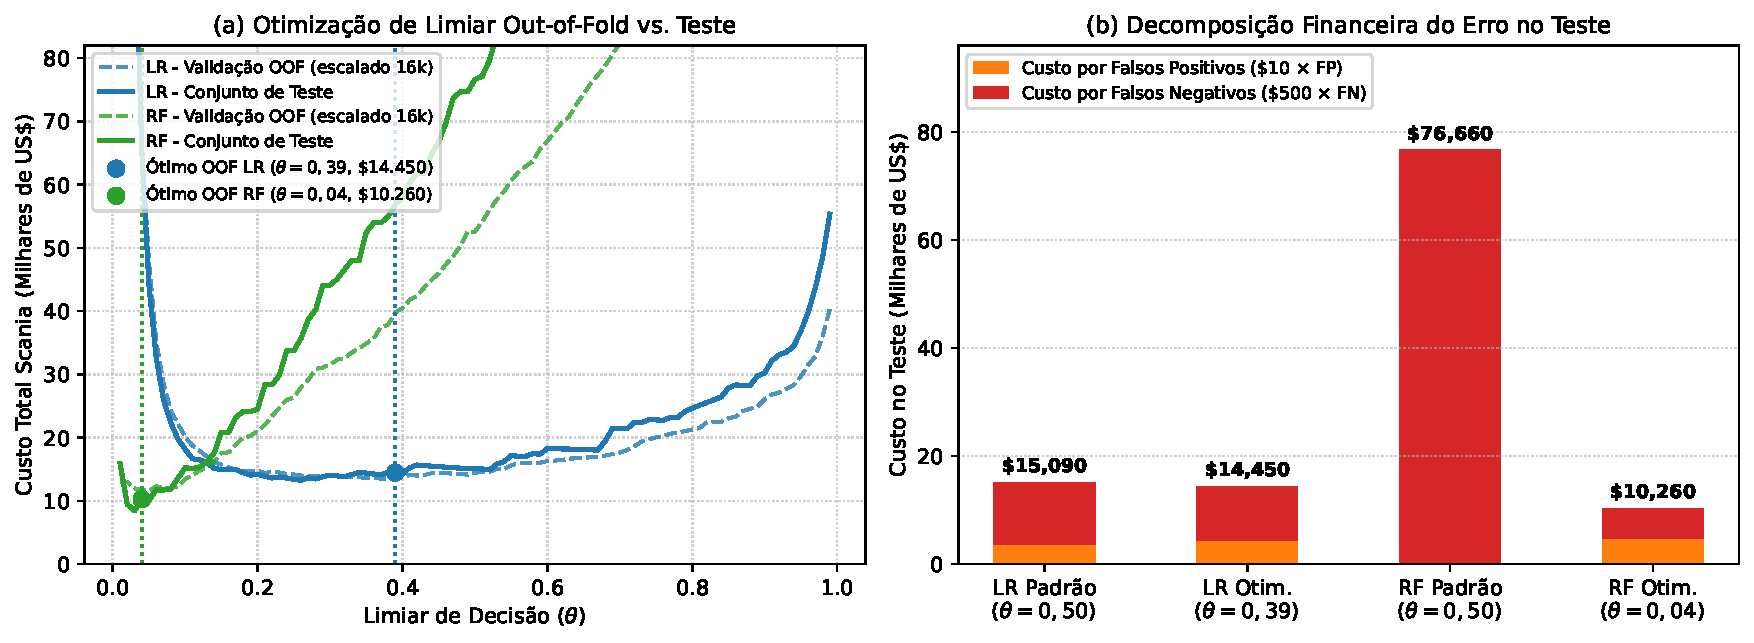
\includegraphics[width=0.96\textwidth]{fig_custo_limiar}
\caption{Avaliação sensível ao custo na estratégia de referência E1: (a) curvas de custo total em função do limiar $\theta$ na validação \textit{out-of-fold} (escalada para 16.000 amostras) e no conjunto de teste cego, destacando a aderência dos pontos ótimos $\theta_{OOF}$; e (b) decomposição financeira do custo no teste entre falsos positivos (\$10 $\times FP$) e falsos negativos (\$500 $\times FN$).}
\label{fig:custo_limiar}
\end{figure*}

A análise crítica da Tabela~\ref{tab:resultados_teste_principal} e da Figura~\ref{fig:custo_limiar} revela comportamentos fundamentais sobre o problema:
\begin{enumerate}
    \item \textbf{O Paradoxo da Acurácia e do $F_1$-Score no Limiar Padrão ($\theta = 0{,}50$):} Com $\theta = 0{,}50$, a \textit{Random Forest} atinge a maior acurácia global (98,94\%), a maior precisão (93,28\%) e o maior $F_1$-Score (0,7243), cometendo apenas 16 alarmes falsos em 15.625 veículos sem falha no APS. Entretanto, sob a ótica operacional da Scania, esse modelo é financeiramente proibitivo: ele deixa escapar $FN = 153$ das 375 falhas reais (\textit{Recall} de apenas 59,20\%), gerando um custo catastrófico de \$76.660 (\$76.500 apenas em quebras em rota). Isso ocorre porque, em árvores profundas com amostras \textit{bootstrap}, cada folha terminal quase pura é determinada por uma subamostra local, e a média dos votos da floresta raramente ultrapassa $0{,}50$ para a classe minoritária (1,67\%), mesmo com \texttt{class\_weight="balanced\_subsample"}.
    \item \textbf{Eficácia do Ajuste de Limiar \textit{Out-of-Fold} ($\theta_{OOF}$):} Ao deslocar o corte de decisão da \textit{Random Forest} para $\theta_{OOF} = 0{,}04$ (ou seja, encaminhar o caminhão à inspeção sempre que ao menos 4 das 100 árvores apontarem falha no APS), o número de falsos negativos cai drasticamente de 153 para apenas 11 em 375 falhas reais (\textit{Recall} de 97,07\%), reduzindo o custo total em 86,6\% (de \$76.660 para \textbf{\$10.260}). Na Regressão Logística, como os pesos balanceados ($\omega_{pos}/\omega_{neg} \approx 59$) já deslocam nativamente o hiperplano linear na função de perda, o modelo já opera razoavelmente bem em $\theta = 0{,}50$ (\$15.090), e o refinamento para $\theta_{OOF} = 0{,}39$ reduz os falsos negativos de 23 para 20 (\textit{Recall} de 94,67\%), diminuindo o custo final para \textbf{\$14.450}.
    \item \textbf{Custo da Interpretabilidade e Leveza Computacional:} Na configuração nominal E1, optar pela Regressão Logística em vez da \textit{Random Forest} implica um custo operacional adicional de \$4.190 no lote de 16.000 veículos (+40,8\%, ou \$0,26 por veículo monitorado), decorrente principalmente de 9 falsos negativos adicionais (20 contra 11) devido à incapacidade do separador linear em capturar interações não lineares entre contadores de uso e caudas de histogramas de pressão. Em contrapartida, a Regressão Logística treina em $2{,}45\text{ s}$ (contra $7{,}13\text{ s}$ da floresta) e realiza a inferência das 16.000 amostras de teste em apenas $3{,}66\text{ ms}$ (contra $48{,}89\text{ ms}$ da \textit{Random Forest}, uma aceleração de $13{,}4\times$), exigindo armazenamento de apenas 163 parâmetros em ponto flutuante.
    \item \textbf{Confronto com Trabalhos Relacionados:} Sem recorrer a geração de dados sintéticos (CGAN ou SMOTE) ou arquiteturas profundas em GPU, a \textit{Random Forest} com ajuste de limiar \textit{out-of-fold} (\$10.260 em E1, chegando a \$9.450 em E4 e \$8.410 com calibração de Platt) supera os resultados reportados por Oh e Lee~\cite{oh2020} (\$31.570 com DNN+GAN), Syed et al.~\cite{syed2020} (\$20.190 com classificador linear próprio) e Rafsunjani et al.~\cite{rafsunjani2019} (\$12.210 com RF e subamostragem), equiparando-se ao XGBoost ponderado de Akarte e Hemachandra~\cite{akarte2018} (\$10.140) e à rede siamesa contrastiva de Sun et al.~\cite{sun2023} (\$9.080). Mesmo o \textit{baseline} de Regressão Logística (\$14.450 em E1 e \$12.910 em E4) supera em mais de \$5.700 o classificador linear especializado de Syed et al.~\cite{syed2020} (\$20.190).
\end{enumerate}

\subsection{Estabilidade sob Diferentes Estratégias de Tratamento de Atributos Ausentes}

Para verificar se a vantagem da \textit{Random Forest} sobre a Regressão Logística e os padrões de erro observados dependem da escolha específica de imputação (E1), a Tabela~\ref{tab:estabilidade_imputacao} e a Figura~\ref{fig:estabilidade_imputacao} apresentam os resultados das cinco estratégias de tratamento de dados ausentes (E1 a E5), todas avaliadas sob o mesmo protocolo de 5 dobras sem vazamento.

\begin{table*}[htbp]
\caption{Análise de Estabilidade sob Diferentes Estratégias de Tratamento de Atributos Ausentes (Validação 5-Fold e Conjunto de Teste)}
\label{tab:estabilidade_imputacao}
\centering
\footnotesize
\begin{tabular}{llccccccccr}
\toprule
& & & \multicolumn{4}{c}{\textbf{Regressão Logística ($C=0{,}01$)}} & \multicolumn{4}{c}{\textbf{Random Forest ($B=100$)}} \\
\cmidrule(lr){4-7} \cmidrule(lr){8-11}
\textbf{Cód.} & \textbf{Estratégia de Tratamento} & \textbf{Atrib.} & $\boldsymbol{\theta_{OOF}}$ & \textbf{Custo Val./Dobra} & $\mathbf{FP / FN}$ & \textbf{Custo Teste} & $\boldsymbol{\theta_{OOF}}$ & \textbf{Custo Val./Dobra} & $\mathbf{FP / FN}$ & \textbf{Custo Teste} \\
\midrule
E1 & Corte $>50\%$ + Mediana (Ref.) & 162 & 0,39 & $10.288 \pm 1.660$ & 445 / 20 & \$14.450 & 0,04 & $8.626 \pm 875$ & 476 / 11 & \$10.260 \\
E2 & Corte $>50\%$ + Média & 162 & 0,34 & $10.392 \pm 1.541$ & 497 / 19 & \$14.470 & 0,05 & $8.370 \pm 1.688$ & 422 / 16 & \$12.220 \\
E3 & Corte $>50\%$ + Constante Zero & 162 & 0,45 & $10.248 \pm 1.667$ & 396 / 25 & \$16.460 & 0,05 & $8.130 \pm 816$ & 412 / 17 & \$12.620 \\
\textbf{E4} & \textbf{Corte $>50\%$ + Mediana + Ind. MNAR} & \textbf{323} & \textbf{0,29} & $\mathbf{9.962 \pm 1.664}$ & \textbf{591 / 14} & \textbf{\$12.910} & \textbf{0,04} & $\mathbf{7.612 \pm 1.090}$ & \textbf{495 / 9} & \textbf{\$9.450} \\
E5 & Sem Corte (170 col.) + Mediana & 170 & 0,28 & $10.396 \pm 1.636$ & 595 / 16 & \$13.950 & 0,04 & $8.808 \pm 1.144$ & 481 / 12 & \$10.810 \\
\bottomrule
\end{tabular}
\end{table*}

\begin{figure}[htbp]
\centering
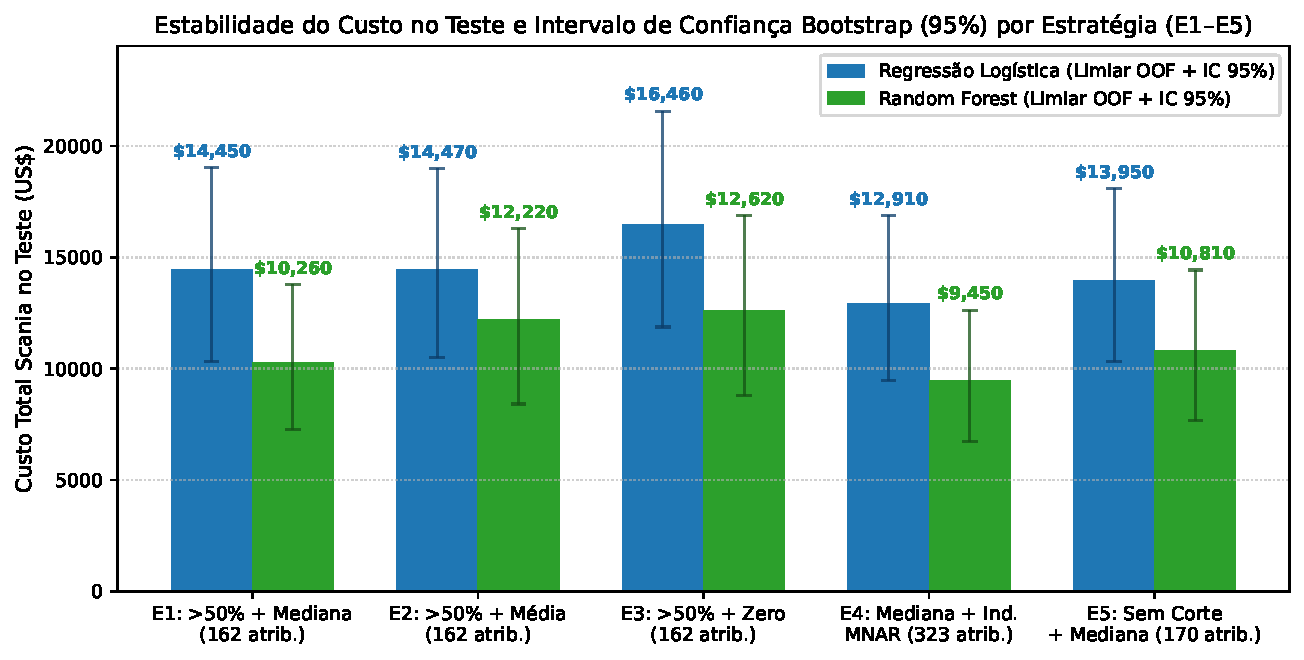
\includegraphics[width=\columnwidth]{fig_estabilidade_imputacao}
\caption{Comparação do custo total no conjunto de teste para a Regressão Logística e a \textit{Random Forest} ao longo das cinco estratégias de tratamento de atributos ausentes (E1 a E5).}
\label{fig:estabilidade_imputacao}
\end{figure}

Os resultados da Tabela~\ref{tab:estabilidade_imputacao} fornecem evidências robustas em três aspectos:
\begin{enumerate}
    \item \textbf{Estabilidade do Ranqueamento entre Famílias de Modelos:} Em todas as cinco estratégias investigadas (E1 a E5), tanto na validação cruzada quanto no teste cego, a \textit{Random Forest} consistentemente alcança menor custo que a Regressão Logística, mantendo uma razão de custo $C_{LR}/C_{RF}$ estável no intervalo entre $1{,}18\times$ (E2) e $1{,}41\times$ (E1). Portanto, a conclusão central sobre a superioridade preditiva do comitê de árvores frente ao modelo linear não é um artefato da escolha de imputação.
    \item \textbf{Superioridade da Mediana (E1) sobre a Média (E2) e Zero (E3):} A substituição da mediana pela média aritmética (E2) praticamente não altera a Regressão Logística (\$14.470 vs. \$14.450), mas degrada o custo da \textit{Random Forest} no teste de \$10.260 para \$12.220 (+5 falsos negativos) e duplica o desvio-padrão nas dobras de validação (de \$875 para \$1.688). Isso se explica pela forte assimetria à direita dos contadores operacionais da Scania, nos quais valores extremos deslocam a média para patamares artificiais que criam divisões espúrias nas árvores de decisão. O preenchimento por zero (E3) apresenta o pior desempenho em ambos os modelos (\$16.460 na Regressão Logística e \$12.620 na \textit{Random Forest}), pois confunde a ausência de medição com leitura física nula de pressão ou temperatura.
    \item \textbf{Valor Preditivo da Ausência Não Aleatória -- Hipótese MNAR (E4 e E5):} A Estratégia E4 (adição de 161 indicadores binários de ausência às 162 variáveis imputadas pela mediana, totalizando 323 atributos) conquista o \textbf{menor custo absoluto tanto na validação quanto no teste para ambos os algoritmos}: o custo da \textit{Random Forest} cai para \textbf{\$9.450} (apenas 9 falsos negativos em 375 falhas reais, \textit{Recall} de 97,60\%) e o da Regressão Logística cai para \textbf{\$12.910} (redução de 20 para 14 falsos negativos, \textit{Recall} de 96,27\%). De forma convergente, manter as 8 colunas altamente incompletas em E5 reduz o custo da Regressão Logística para \$13.950 frente a E1 (\$14.450). Esses dois achados comprovam empiricamente que a ausência de dados no APS Failure é informativa (MNAR): o padrão de quais sensores deixaram de reportar ajuda os classificadores a isolar caminhões com falha severa no sistema pneumático.
\end{enumerate}

\subsection{Impacto da Calibração de Probabilidades e Limiar Teórico de Bayes}

A Tabela~\ref{tab:calibracao_probabilidades} e a Figura~\ref{fig:calibracao_probabilidades} examinam o efeito da calibração pós-treinamento (\textit{Platt Scaling} sigmoidal e Regressão Isotônica via PAVA) sobre a qualidade das probabilidades estimadas (mensurada pelo Brier Score e pela probabilidade média predita no teste, cuja prevalência real de positivos é $375/16.000 = 0{,}0234$) e confrontam duas políticas de escolha de limiar: a aplicação direta do limiar ótimo teórico de Bayes ($\theta^* = 10/510 \approx 0{,}0196$) versus o limiar empírico otimizado \textit{out-of-fold} ($\theta_{OOF}$).

\begin{table*}[htbp]
\caption{Impacto da Calibração de Probabilidades sobre o Brier Score e sobre o Custo no Teste com Limiar de Bayes ($\theta^* = 0{,}0196$) vs. Limiar Empírico ($\theta_{OOF}$)}
\label{tab:calibracao_probabilidades}
\centering
\footnotesize
\begin{tabular}{llcccccccc}
\toprule
& & & & \multicolumn{3}{c}{\textbf{Regra Teórica de Bayes ($\boldsymbol{\theta^* = 0{,}0196}$)}} & \multicolumn{3}{c}{\textbf{Limiar Otimizado OOF ($\boldsymbol{\theta_{OOF}}$)}} \\
\cmidrule(lr){5-7} \cmidrule(lr){8-10}
\textbf{Modelo Base} & \textbf{Método de Calibração} & \textbf{Brier (Teste)} & $\boldsymbol{\bar{\hat{P}}}$ \textbf{(Teste)} & $\mathbf{FP / FN}$ & \textbf{Recall} & \textbf{Custo Bayes} & $\boldsymbol{\theta_{OOF}}$ & $\mathbf{FP / FN}$ & \textbf{Custo OOF} \\
\midrule
Reg. Logística & Sem Calibração (\texttt{balanced}) & 0,02182 & 0,0878 & 14.368 / 1 & 0,9973 & \$144.180 & 0,39 & 445 / 20 & \$14.450 \\
Reg. Logística & Escalonamento de Platt & 0,00975 & 0,0215 & 340 / 23 & 0,9387 & \$14.900 & 0,01 & 638 / 14 & \textbf{\$13.380} \\
Reg. Logística & Regressão Isotônica (PAVA) & \textbf{0,00875} & \textbf{0,0212} & \textbf{434 / 20} & \textbf{0,9467} & \textbf{\$14.340} & \textbf{0,03} & \textbf{434 / 20} & \textbf{\$14.340} \\
\midrule
Random Forest & Sem Calibração (\texttt{balanced\_sub.}) & 0,00774 & 0,0180 & 793 / 3 & 0,9920 & \$9.430 & 0,04 & 476 / 11 & \$10.260 \\
Random Forest & Escalonamento de Platt & 0,00696 & 0,0204 & \textbf{591 / 5} & \textbf{0,9867} & \textbf{\$8.410} & 0,04 & 476 / 11 & \$10.260 \\
Random Forest & Regressão Isotônica (PAVA) & \textbf{0,00683} & \textbf{0,0208} & 476 / 11 & 0,9707 & \$10.260 & \textbf{0,02} & \textbf{476 / 11} & \$10.260 \\
\bottomrule
\end{tabular}
\end{table*}

\begin{figure*}[htbp]
\centering
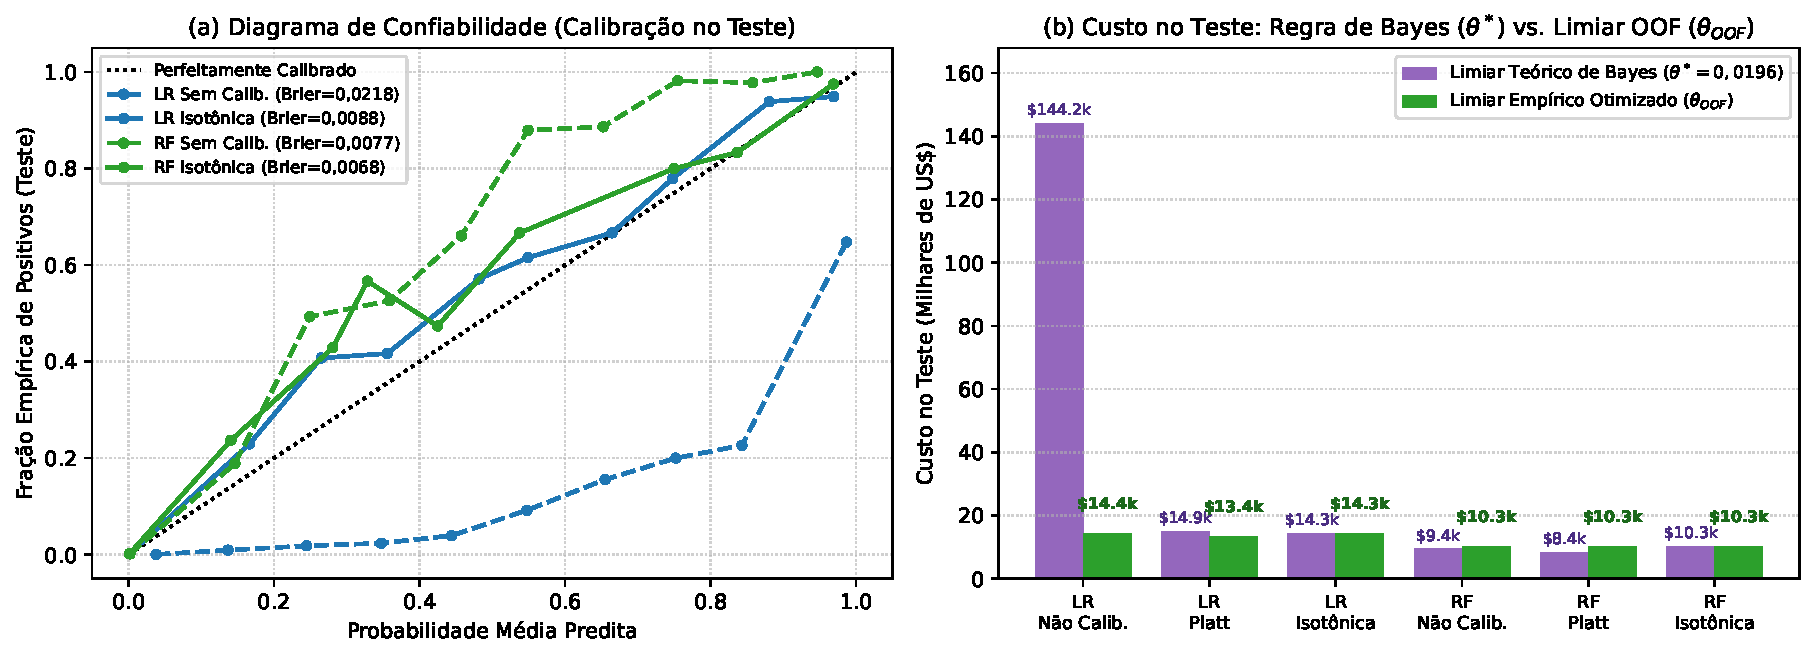
\includegraphics[width=0.96\textwidth]{fig_calibracao_probabilidades}
\caption{Análise de calibração de probabilidades no conjunto de teste: (a) diagrama de confiabilidade comparando as estimativas não calibradas e calibradas via Regressão Isotônica frente à diagonal ideal; e (b) impacto da calibração sobre o custo financeiro ao aplicar diretamente o limiar teórico de Bayes ($\theta^* = 0{,}0196$) em comparação ao limiar empírico $\theta_{OOF}$.}
\label{fig:calibracao_probabilidades}
\end{figure*}

A análise conjunta da Tabela~\ref{tab:calibracao_probabilidades} e da Figura~\ref{fig:calibracao_probabilidades} elucida o papel decisivo da calibração probabilística:
\begin{enumerate}
    \item \textbf{Correção da Distorção Induzida pelo Balanceamento de Classes:} Na Regressão Logística sem calibração, a ponderação $\omega_{pos}/\omega_{neg} \approx 59$ infla severamente as probabilidades preditas: a probabilidade média atribuída no teste é $\bar{\hat{P}} = 0{,}0878$ (quase quatro vezes superior à taxa real de falhas de $0{,}0234$), resultando em uma curva de confiabilidade fortemente deslocada abaixo da diagonal ideal (Figura~\ref{fig:calibracao_probabilidades}a) e em um Brier Score elevado ($0{,}02182$). Se um engenheiro aplicasse diretamente a regra teórica de Bayes ($\theta^* = 0{,}0196$) a esse modelo não calibrado, o classificador geraria 14.368 falsos positivos (mandando 92\% da frota saudável para a oficina) a um custo exorbitante de \$144.180. Após a calibração por Regressão Isotônica ou \textit{Platt Scaling}, o Brier Score cai mais de 55\% (para $0{,}00875$ e $0{,}00975$), a probabilidade média converge para a prevalência real ($0{,}0212$ e $0{,}0215$), e o uso direto do limiar teórico $\theta^* = 0{,}0196$ reduz o custo de \$144.180 para \textbf{\$14.340} (Isotônica) e \$14.900 (Platt), enquanto o ajuste $\theta_{OOF}$ sobre Platt alcança \$13.380.
    \item \textbf{Convergência entre o Limiar Empírico ($\theta_{OOF}$) e o Limiar de Bayes ($\theta^*$) após Calibração:} Observa-se que, antes da calibração, o limiar empírico ótimo da Regressão Logística era $\theta_{OOF} = 0{,}39$, muito distante de $\theta^* = 0{,}0196$. Uma vez calibradas as probabilidades pela Regressão Isotônica, o limiar ótimo empírico desloca-se exatamente para $\theta_{OOF} = 0{,}03$ (na Regressão Logística) e $\theta_{OOF} = 0{,}02$ (na \textit{Random Forest}), coincidindo com o valor teórico de Bayes ($\theta^* \approx 0{,}02$) e produzindo o exato mesmo custo no teste (\$14.340 e \$10.260). Isso valida na prática a teoria de Zadrozny e Elkan~\cite{zadrozny2002transforming} e Dal Pozzolo et al.~\cite{dalpozzolo2015calibrating}: quando o classificador é devidamente calibrado para a distribuição real da frota, a regra analítica de risco mínimo de Bayes torna-se diretamente aplicável.
    \item \textbf{Ganho Adicional do Escalonamento de Platt na \textit{Random Forest}:} Na \textit{Random Forest}, a calibração paramétrica de Platt reduz o Brier Score de $0{,}00774$ para $0{,}00696$ e suaviza a cauda inferior de probabilidades (onde a grade discreta de 100 árvores possui resolução limitada a saltos de $0{,}01$). Como resultado, ao aplicar o limiar de Bayes $\theta^* = 0{,}0196$ sobre as probabilidades contínuas calibradas por Platt, o modelo detecta 370 das 375 falhas reais ($FN = 5$, \textit{Recall} de 98,67\%) com 591 falsos positivos, atingindo o custo notável de \textbf{\$8.410} no conjunto de teste.
\end{enumerate}

\subsection{Análise de Sensibilidade aos Custos Atribuídos aos Erros}

Em cenários reais de operação logística, a razão $\rho = c_{FN}/c_{FP}$ entre o custo de uma avaria na estrada e o custo de uma inspeção preventiva varia conforme o valor da carga, multas por atraso e disponibilidade de oficinas. A Tabela~\ref{tab:sensibilidade_custos} e a Figura~\ref{fig:sensibilidade_custos} apresentam a análise de sensibilidade variando $\rho \in \{10, 25, 50, 100, 200\}$ (com $c_{FP} = \$10$ fixo e $c_{FN} \in \{\$100, \$250, \$500, \$1.000, \$2.000\}$), reportando também o custo normalizado em relação ao classificador trivial ótimo $C_{trivial} = \min(c_{FP} N_{neg}, c_{FN} N_{pos})$~\cite{drummond2006cost}.

\begin{table*}[htbp]
\caption{Análise de Sensibilidade à Razão de Custos $\rho = c_{FN}/c_{FP}$ no Conjunto de Teste ($c_{FP} = \$10$ Fixo)}
\label{tab:sensibilidade_custos}
\centering
\footnotesize
\begin{tabular}{cccccccccccr}
\toprule
& & & & \multicolumn{3}{c}{\textbf{Regressão Logística ($\boldsymbol{\theta_{OOF}}$)}} & \multicolumn{3}{c}{\textbf{Random Forest ($\boldsymbol{\theta_{OOF}}$)}} & \textbf{RF Isotônica} & \\
\cmidrule(lr){5-7} \cmidrule(lr){8-10} \cmidrule(lr){11-11}
$\boldsymbol{\rho}$ & $\mathbf{c_{FN}}$ & $\boldsymbol{\theta^*}$ \textbf{(Bayes)} & $\mathbf{C_{trivial}}$ & $\boldsymbol{\theta_{OOF}}$ & $\mathbf{FP / FN}$ & \textbf{Custo (\% Triv.)} & $\boldsymbol{\theta_{OOF}}$ & $\mathbf{FP / FN}$ & \textbf{Custo (\% Triv.)} & \textbf{Custo ($\boldsymbol{\theta^*}$)} & \textbf{Razão LR/RF} \\
\midrule
$10:1$ & \$100 & 0,0909 & \$37.500 & 0,67 & 253 / 31 & \$5.630 (15,0\%) & 0,12 & 187 / 27 & \$4.570 (12,2\%) & \$4.570 & $1{,}23\times$ \\
$25:1$ & \$250 & 0,0385 & \$93.750 & 0,39 & 445 / 20 & \$9.450 (10,1\%) & 0,05 & 410 / 12 & \$7.100 (7,6\%) & \$7.100 & $1{,}33\times$ \\
$\mathbf{50:1}$ & \textbf{\$500} & \textbf{0,0196} & \textbf{\$156.250} & \textbf{0,39} & \textbf{445 / 20} & \textbf{\$14.450 (9,2\%)} & \textbf{0,04} & \textbf{476 / 11} & \textbf{\$10.260 (6,6\%)} & \textbf{\$10.260} & $\mathbf{1{,}41\times}$ \\
$100:1$ & \$1.000 & 0,0099 & \$156.250 & 0,16 & 944 / 11 & \$20.440 (13,1\%) & 0,02 & 793 / 3 & \$10.930 (7,0\%) & \$10.930 & $1{,}87\times$ \\
$200:1$ & \$2.000 & 0,0050 & \$156.250 & 0,14 & 1.064 / 9 & \$28.640 (18,3\%) & 0,02 & 793 / 3 & \$13.930 (8,9\%) & \$13.930 & $2{,}06\times$ \\
\bottomrule
\end{tabular}
\end{table*}

\begin{figure*}[htbp]
\centering
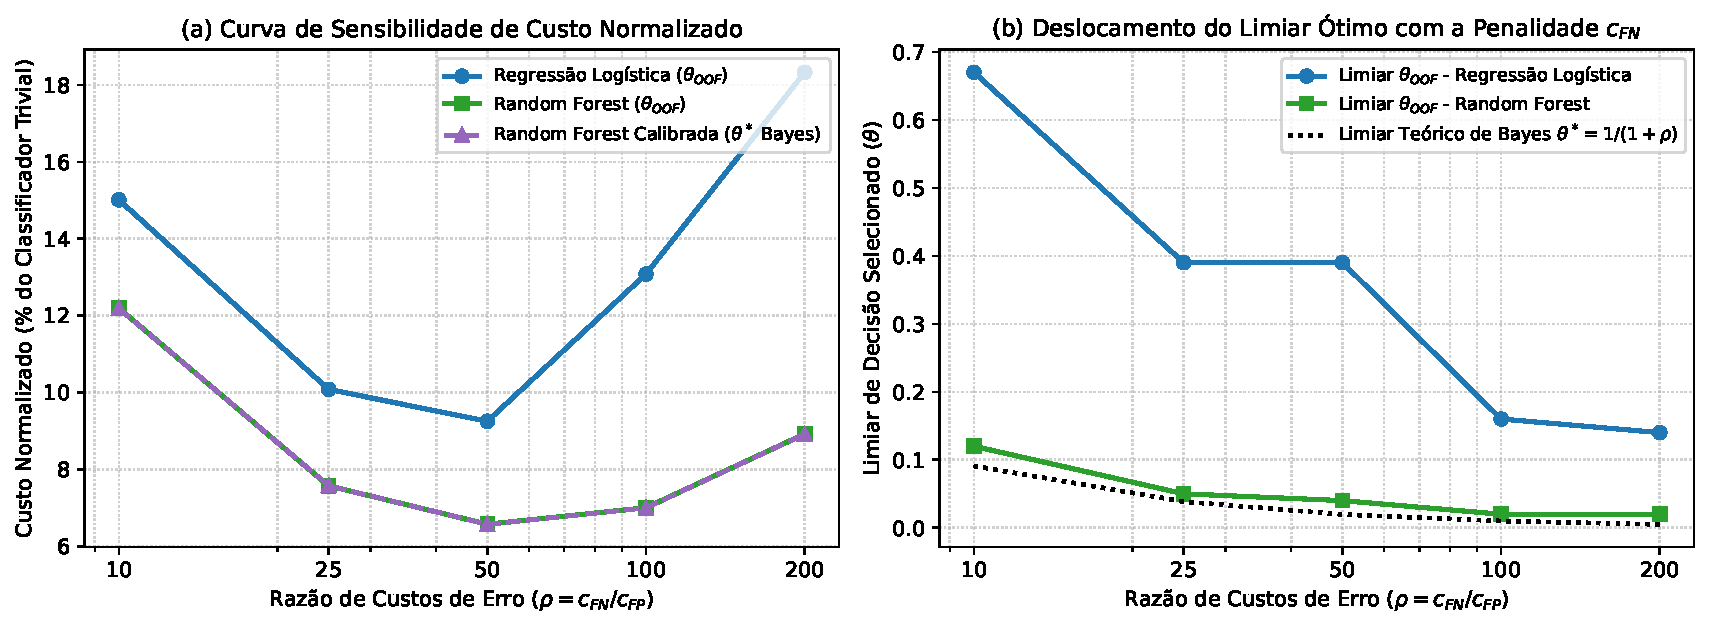
\includegraphics[width=0.96\textwidth]{fig_sensibilidade_custos}
\caption{Análise de sensibilidade à razão de custos $\rho = c_{FN}/c_{FP} \in \{10, 25, 50, 100, 200\}$: (a) custo total no teste normalizado pelo custo do classificador trivial ($C_{trivial}$), evidenciando o alargamento da vantagem da \textit{Random Forest} em regimes de alta penalidade; e (b) adaptação monotônica dos limiares ótimos $\theta_{OOF}$ e $\theta^*$ à medida que a severidade da falha aumenta.}
\label{fig:sensibilidade_custos}
\end{figure*}

A análise de sensibilidade (Tabela~\ref{tab:sensibilidade_custos} e Figura~\ref{fig:sensibilidade_custos}) revela três conclusões de grande relevância prática para a gestão de manutenção:
\begin{enumerate}
    \item \textbf{Regime de Penalidade Moderada ($\rho \in [10, 25]$):} Quando o custo de falha em rota é de 10 a 25 vezes o custo de inspeção, a diferença relativa entre a Regressão Logística e a \textit{Random Forest} é reduzida: em $\rho = 10$, a Regressão Logística custa \$5.630 contra \$4.570 da \textit{Random Forest} (sobrecusto de apenas \$1.060 no lote de 16.000 caminhões, ou razão de $1{,}23\times$). Nesse regime, alinhado à análise teórica de Hughes, Perinpanayagam e Ball~\cite{hughes2025xai}, o baixo sobrecusto financeiro justifica plenamente a adoção do modelo linear caso a equipe de engenharia priorize transparência nos pesos dos sensores ou execução embarcada em microcontroladores veiculares.
    \item \textbf{Regime de Penalidade Severa ($\rho \in [100, 200]$):} À medida que a penalidade por falso negativo cresce para \$1.000 ($\rho = 100$) e \$2.000 ($\rho = 200$), os classificadores precisam operar no extremo de alta sensibilidade (\textit{Recall} $> 97\%$). Para reduzir seus falsos negativos de 20 para 9, a Regressão Logística precisa baixar seu limiar para $\theta_{OOF} = 0{,}14$, o que faz seus falsos positivos saltarem para 1.064, elevando o custo para \$28.640 (18,3\% do custo trivial). Já a \textit{Random Forest}, ao adotar $\theta_{OOF} = 0{,}02$, consegue reter apenas $FN = 3$ falhas não detectadas em todo o conjunto de teste (\textit{Recall} de 99,20\%) com 793 falsos positivos, mantendo o custo em \$10.930 ($\rho=100$) e \$13.930 ($\rho=200$, apenas 8,9\% do custo trivial). Assim, o sobrecusto relativo da Regressão Logística dobra, subindo de $1{,}23\times$ para **$2{,}06\times$**.
    \item \textbf{Exatidão da Regra de Bayes sem Reajuste Empírico:} A penúltima coluna da Tabela~\ref{tab:sensibilidade_custos} e a curva tracejada roxa da Figura~\ref{fig:sensibilidade_custos}a demonstram que a \textit{Random Forest} calibrada por Regressão Isotônica, operando puramente com o limiar analítico $\theta^*(\rho) = 1/(1+\rho)$ sem necessidade de reexecutar busca empírica de limiar a cada mudança de contrato logístico, iguala o custo ótimo da \textit{Random Forest} ($\theta_{OOF}$) em todos os cinco regimes de custo avaliados.
\end{enumerate}

% =========================================================================
% SEÇÃO V: CONCLUSÕES, LIMITAÇÕES E TRABALHOS FUTUROS
% =========================================================================
\section{Conclusões, Limitações da Abordagem e Trabalhos Futuros}
\label{sec:conclusoes}

\subsection{Síntese das Contribuições e Principais Achados}

Este trabalho investigou o diagnóstico preditivo de falhas no Sistema de Pressão de Ar (APS) de caminhões pesados na base pública \textit{APS Failure at Scania Trucks}, contrastando um modelo linear transparente e computacionalmente leve (Regressão Logística com ponderação balanceada de classes) e um comitê não linear de árvores de decisão (\textit{Random Forest}) sob um protocolo experimental estrito de validação cruzada estratificada sem vazamento de dados. Respondendo diretamente à questão de pesquisa sobre o compromisso entre interpretabilidade e eficiência econômica sob custos assimétricos, os resultados experimentais permitem consolidar quatro conclusões principais:
\begin{enumerate}
    \item \textbf{Necessidade Crítica da Otimização de Limiar Orientada ao Custo:} Métricas convencionais avaliadas no limiar padrão ($\theta = 0{,}50$) são enganosas sob desbalanceamento severo ($59:1$). A \textit{Random Forest} padrão obtém 98,94\% de acurácia, mas incorre em \$76.660 de custo por omitir 40,8\% das falhas reais. O ajuste de limiar nas probabilidades \textit{out-of-fold} do treino ($\theta_{OOF} = 0{,}04$) reduz o custo no teste em 86,6\%, atingindo \$10.260 (\textit{Recall} de 97,07\%), ao passo que a Regressão Logística otimizada ($\theta_{OOF} = 0{,}39$) atinge \$14.450 (\textit{Recall} de 94,67\%), com inferência $13{,}4\times$ mais rápida.
    \item \textbf{Estabilidade frente à Imputação e Caráter Informativo da Ausência (MNAR):} A vantagem da \textit{Random Forest} sobre a Regressão Logística manteve-se invariante em todas as cinco estratégias de tratamento de atributos ausentes avaliadas. Demonstrou-se que a imputação pela mediana supera a média e o preenchimento por zero, e que a adição de indicadores binários de ausência (Estratégia E4) reduz significativamente o custo de ambos os modelos (para \$9.450 na \textit{Random Forest} e \$12.910 na Regressão Logística), confirmando que o próprio padrão de omissão dos sensores carrega sinal preditivo sobre a falha.
    \item \textbf{Papel da Calibração Probabilística na Decisão de Risco Mínimo:} Comprovou-se que a ponderação de classes distorce severamente as probabilidades brutas da Regressão Logística (Brier Score de $0{,}02182$), tornando desastrosa a aplicação direta do limiar teórico de Bayes ($\theta^* = 0{,}0196$, custo de \$144.180). A calibração pós-treinamento via Regressão Isotônica e \textit{Platt Scaling} corrige essa distorção (Brier Score de $0{,}00875$), reconciliando o limiar ótimo empírico com o limiar teórico de Bayes (\$14.340) e permitindo que a \textit{Random Forest} calibrada por Platt alcance o menor custo global do estudo (\textbf{\$8.410}).
    \item \textbf{Fronteira de Viabilidade Operacional na Análise de Sensibilidade:} A varredura da razão de custos $\rho = c_{FN}/c_{FP} \in [10, 200]$ mostrou que o modelo linear interpretável impõe um sobrecusto moderado em regimes de baixa razão de penalidade ($1{,}23\times$ para $\rho = 10$), mas torna-se economicamente desfavorável em operações críticas de alta penalidade ($2{,}06\times$ para $\rho = 200$), nas quais a maior precisão da \textit{Random Forest} na cauda extrema de sensibilidade é indispensável.
\end{enumerate}

\subsection{Limitações da Abordagem}

Não obstante a consistência empírica alcançada, reconhecem-se as seguintes limitações metodológicas e práticas do estudo:
\begin{itemize}
    \item \textbf{Anonimização Semântica dos Atributos:} Como os 170 atributos da base da Scania são anonimizados por sigilo industrial, a interpretabilidade intrínseca da Regressão Logística fica restrita à identificação matemática dos códigos das variáveis de maior peso (ex.: \texttt{aa\_000}, \texttt{ci\_000}), impedindo a validação física direta com grandezas termodinâmicas ou pneumáticas específicas (como pressão do compressor ou temperatura da válvula secadora).
    \item \textbf{Natureza Estática e Agregada das Instâncias:} A base APS Failure fornece recortes tabulares agregados por veículo, sem carimbo de tempo (\textit{timestamp}) ou identificação longitudinal de múltiplos registros de um mesmo caminhão ao longo do tempo, o que impossibilita modelar a trajetória contínua de degradação ou estimar a Vida Útil Remanescente (\textit{Remaining Useful Life} -- RUL) em dias ou quilômetros.
    \item \textbf{Discretização da Probabilidade em Comitês Pequenos:} Com $B = 100$ árvores e limiares ótimos situados na faixa muito baixa ($\theta \in [0{,}01; 0{,}05]$), as probabilidades brutas da \textit{Random Forest} sofrem discretização em degraus de $0{,}01$, tornando a decisão sensível a variações de uma única árvore caso não se utilize calibração contínua como o escalonamento de Platt.
    \item \textbf{Escopo de Imputação e Família de Modelos:} O estudo concentrou-se em imputadores univariados rápidos (mediana, média e zero com indicadores binários) e em duas famílias clássicas de classificadores, não incluindo imputação multivariada iterativa (MICE) em razão de seu custo cúbico por atributo, nem comitês de \textit{gradient boosting} com perdas customizadas.
\end{itemize}

\subsection{Trabalhos Futuros}

Como desdobramentos diretos para superar as limitações identificadas, propõem-se quatro direções de pesquisa futura:
\begin{enumerate}
    \item \textbf{Incorporação de Modelos de \textit{Gradient Boosting} com Perda Assimétrica Direta:} Avaliar algoritmos como LightGBM, XGBoost e CatBoost incorporando a matriz de custos $(c_{FP}, c_{FN})$ diretamente no gradiente e no hessiano da função objetivo de treinamento (ou via \textit{focal loss} calibrada), comparando-os ao ajuste de limiar pós-hoc.
    \item \textbf{Explicabilidade Pós-Hoc Local e Global (XAI):} Aplicar valores de Shapley (\textit{TreeSHAP}) sobre a \textit{Random Forest} calibrada com indicadores MNAR (E4) para extrair explicações locais por caminhão inspecionado, combinando o baixo custo operacional das árvores (\$8.410--\$9.450) com transparência diagnóstica auditável em oficina~\cite{hughes2025xai}.
    \item \textbf{Extensão para Séries Temporais na Base \textit{SCANIA Component X}:} Transferir o protocolo de calibração probabilística e análise de sensibilidade de custos para o conjunto longitudinal \textit{SCANIA Component X}~\cite{twostage2025}, integrando janelas deslizantes temporais para previsão de tempo até a falha.
    \item \textbf{Amostragem Híbrida e Imputação Multivariada Leve:} Investigar o acoplamento dos indicadores binários MNAR com imputação por $k$-vizinhos mais próximos ($k$-NN) ou fatoração matricial de baixo posto, verificando se a combinação reduz ainda mais os 5 a 9 falsos negativos residuais observados no conjunto de teste.
\end{enumerate}

% =========================================================================
% REFERÊNCIAS BIBLIOGRÁFICAS (PADRÃO IEEE)
% =========================================================================
\begin{thebibliography}{00}

\bibitem{hector2024predictive}
I.~Hector and R.~Panjanathan, ``Predictive maintenance in Industry 4.0: a survey of planning models and machine learning techniques,'' \emph{PeerJ Computer Science}, vol.~10, p.~e2016, 2024, doi: \href{https://doi.org/10.7717/peerj-cs.2016}{10.7717/peerj-cs.2016}.

\bibitem{rengasamy2020deep}
D.~Rengasamy, M.~Jafari, B.~Rothwell, X.~Chen, and G.~P.~Figueredo, ``Deep learning with dynamically weighted loss function for sensor-based prognostics and health management,'' \emph{Sensors}, vol.~20, no.~3, p.~723, 2020.

\bibitem{gondek2016prediction}
C.~Gondek, D.~Hafner, and O.~R.~Sampson, ``Prediction of failures in the air pressure system of Scania trucks using a random forest and feature engineering,'' in \emph{Advances in Intelligent Data Analysis XV}, pp.~398--402, Springer, 2016.

\bibitem{cerqueira2016combining}
V.~Cerqueira, F.~Pinto, C.~Sá, and C.~Soares, ``Combining boosted trees with metafeature engineering for predictive maintenance,'' in \emph{Advances in Intelligent Data Analysis XV}, pp.~393--397, Springer, 2016.

\bibitem{costa2016ida}
C.~F.~Costa and M.~A.~Nascimento, ``IDA 2016 Industrial Challenge: Using machine learning for predicting failures,'' in \emph{Advances in Intelligent Data Analysis XV (Lecture Notes in Computer Science)}, vol. 9897, pp.~381--386, Springer, 2016.

\bibitem{scania_dataset}
Scania CV AB, ``APS Failure at Scania Trucks Dataset,'' \emph{UCI Machine Learning Repository}, 2017, doi: \href{https://doi.org/10.24432/C51851}{10.24432/C51851}. [Online]. Disponível em: \url{https://archive.ics.uci.edu/dataset/421/aps+failure+at+scania+trucks}.

\bibitem{costtransformer2024}
A.~Beikmohammadi, M.~H.~Hamian, N.~Khoeyniha, T.~Lindgren, O.~Steinert, and S.~Magn\'usson, ``A cost-sensitive transformer model for prognostics under highly imbalanced industrial data,'' arXiv:2402.08611, 2024.

\bibitem{akarte2018}
M.~M.~Akarte and N.~Hemachandra, ``Predictive maintenance of air pressure system using boosting trees: A machine learning approach,'' in \emph{ORSI}, 2018.

\bibitem{rafsunjani2019}
S.~Rafsunjani, R.~S.~Safa, A.~Al Imran, M.~S.~Rahim, and D.~Nandi, ``An empirical comparison of missing value imputation techniques on APS failure prediction,'' \emph{Int. J. Inf. Technol. Comput. Sci.}, vol.~2, pp.~21--29, 2019.

\bibitem{ranasinghe2019}
G.~D.~Ranasinghe, T.~Lindgren, M.~Girolami, and A.~K.~Parlikad, ``A methodology for prognostics under the conditions of limited failure data availability,'' \emph{IEEE Access}, vol.~7, pp.~183996--184007, 2019.

\bibitem{syed2020}
M.~N.~Syed, M.~R.~Hassan, I.~Ahmad, M.~M.~Hassan, and V.~H.~C.~De Albuquerque, ``A novel linear classifier for class imbalance data arising in failure-prone air pressure systems,'' \emph{IEEE Access}, vol.~9, pp.~4211--4222, 2020.

\bibitem{oh2020}
E.~Oh and H.~Lee, ``An imbalanced data handling framework for industrial big data using a Gaussian process regression-based generative adversarial network,'' \emph{Symmetry}, vol.~12, no.~4, p.~669, 2020.

\bibitem{sun2023}
K.~Sun, S.~Magn\'usson, O.~Steinert, and T.~Lindgren, ``Robust contrastive learning and multi-shot voting for high-dimensional multivariate data-driven prognostics,'' in \emph{Proc. IEEE Int. Conf. Prognostics and Health Management (ICPHM)}, 2023, pp.~53--60.

\bibitem{twostage2025}
S.-W.~Kim and Y.~S.~Kim, ``Two-stage LightGBM framework for cost-sensitive prediction of impending failures of Component X in Scania trucks,'' \emph{Computers, Materials \& Continua}, vol.~86, no.~3, art.~50, 2026, doi: \href{https://doi.org/10.32604/cmc.2025.073492}{10.32604/cmc.2025.073492}.

\bibitem{costopt2025}
Y.~Yang and M.~Z.~Iqbal, ``Cost-optimised machine learning model comparison for predictive maintenance,'' \emph{Electronics}, vol.~14, no.~12, art.~2497, 2025, doi: \href{https://doi.org/10.3390/electronics14122497}{10.3390/electronics14122497}.

\bibitem{hughes2025xai}
P.~Hughes, S.~Perinpanayagam, and P.~D.~Ball, ``Cost-efficiency and cost-effectiveness of XAI in predictive maintenance,'' \emph{IEEE Access}, pp.~151664--151670, 2025, doi: \href{https://doi.org/10.1109/ACCESS.2025.3601385}{10.1109/ACCESS.2025.3601385}.

\bibitem{elkan2001foundations}
C.~Elkan, ``The foundations of cost-sensitive learning,'' in \emph{Proc. 17th Int. Joint Conf. on Artificial Intelligence (IJCAI)}, 2001, pp.~973--978.

\bibitem{zadrozny2002transforming}
B.~Zadrozny and C.~Elkan, ``Transforming classifier scores into accurate multiclass probability estimates,'' in \emph{Proc. 8th ACM SIGKDD Int. Conf. on Knowledge Discovery and Data Mining (KDD)}, 2002, pp.~694--699.

\bibitem{niculescu2005predicting}
A.~Niculescu-Mizil and R.~Caruana, ``Predicting good probabilities with supervised learning,'' in \emph{Proc. 22nd Int. Conf. on Machine Learning (ICML)}, 2005, pp.~625--632.

\bibitem{dalpozzolo2015calibrating}
A.~Dal~Pozzolo, O.~Caelen, R.~A.~Johnson, and G.~Bontempi, ``Calibrating probability with undersampling for unbalanced classification,'' in \emph{Proc. IEEE Symp. Series on Computational Intelligence (SSCI)}, 2015, pp.~159--166.

\bibitem{drummond2006cost}
C.~Drummond and R.~C.~Holte, ``Cost curves: An improved method for visualizing classifier performance,'' \emph{Machine Learning}, vol.~65, no.~1, pp.~95--130, 2006.

\end{thebibliography}

\end{document}
